\chapter{Założenia projektowe}
\section{Reguły i mechanika gry}
Gra stworzona w ramach projektu będzie nazywała się \emph{Sunset Showdown}. Charakterystyczne dla gry będzie ujednolicenie postaci sterowanymi przez graczy. Każda z postaci będzie miała 3 punkty zdrowia, a zwycięstwo w rundzie będzie osiągane poprzez zredukowanie zdrowia przeciwnika do zera. W przypadku trzykrotnego powodzenia tego procesu, gracz wygrywa całą grę. 

Postacie będą miały możliwość zadawania ciosów na trzech różnych wysokościach: \emph{high} (cios wysoki), \emph{mid} (cios wyprowadzony w środkową część ciała) oraz \emph{low} (cios niski). Wysokość ciosu wpływa na to, w jakim stanie można go zablokować lub uniknąć. Cios \emph{high} można zablokować stojąc, uniknąć zaś kucając. Cios \emph{mid} można zablokować w pozycji stojącej, jednak nie chroni przed nim kucanie. Natomiast ciosem \emph{low} można trafić stojącego przeciwnika, przy czym może on go zablokować kucając. 

Dodatkowo, każdy cios będzie charakteryzować się inną szybkością. Atak \emph{high} będzie najszybszy, \emph{mid} zajmie środkową pozycję, natomiast cios \emph{low} będzie najwolniejszy. 

Każdy atak zadaje określoną ilość obrażeń (\emph{high} -- 3 obr., \emph{mid} -- 2 obr., \emph{low} -- 1 obr.). Dodatkowo każdy cios będzie powodował inną animację u przeciwnika na bloku (tzw.~\emph{blockstun}), od której będzie zależało, jak będzie wyglądała sytuacja po zablokowanym ataku. Po zablokowaniu ataku \emph{high}, atakujący znajduje się w lepszej pozycji, gdyż \emph{blockstun} trwa na tyle długo, że atakujący będzie mógł szybciej odzyskać kontrolę nad postacią. W przypadku ataku \emph{mid}, sytuacja odwraca się, a po zablokowaniu obrońca znajduje się w lepszej pozycji. Sytuacja po zablokowaniu ciosu \emph{low} jest szczególnie dynamiczna, ponieważ blokujący ma wystarczająco dużo czasu, aby zareagować ciosem \emph{high}, co równa się z wygraniem rundy (tzw.~\emph{block punishment}).

Wszystkie kluczowe informacje na temat ciosów postaci znajdują się w tabeli~\ref{tab:ataki}. Wartości szybkości ruchów i sytuacji zarówno na trafieniu i na bloku są podawane w ,,klatkach'', które są równoznaczne z 1/60 sekundy (np.\ jeżeli sytuacja na trafieniu wynosi +2 oznacza to że postać atakującego po trafieniu będzie mogła wrócić do kontroli nad swoją postacią o 2/60 sekundy szybciej niż przeciwnik).

\begin{table}[htb] \small
\centering
\caption{Atrybuty ataków dostępnych dla postaci}
\label{tab:ataki}
\begin{tabularx}{\linewidth}{|c|X|X|X|X|} \hline\
Wysokość ataku & Szybkość ataku & Obrażenia & Sytuacja na bloku & Sytuacja na trafieniu \\ \hline\hline
\texttt{high} & 15 & 3 & +1 & nie dotyczy \\ \hline
\texttt{mid} & 18 & 2 & -2 & +2\\ \hline
\texttt{low} & 21 & 1 & -15 & +2\\ \hline
\end{tabularx}
\end{table}

\section{Interfejs użytkownika}
\begin{figure}
	\centering
		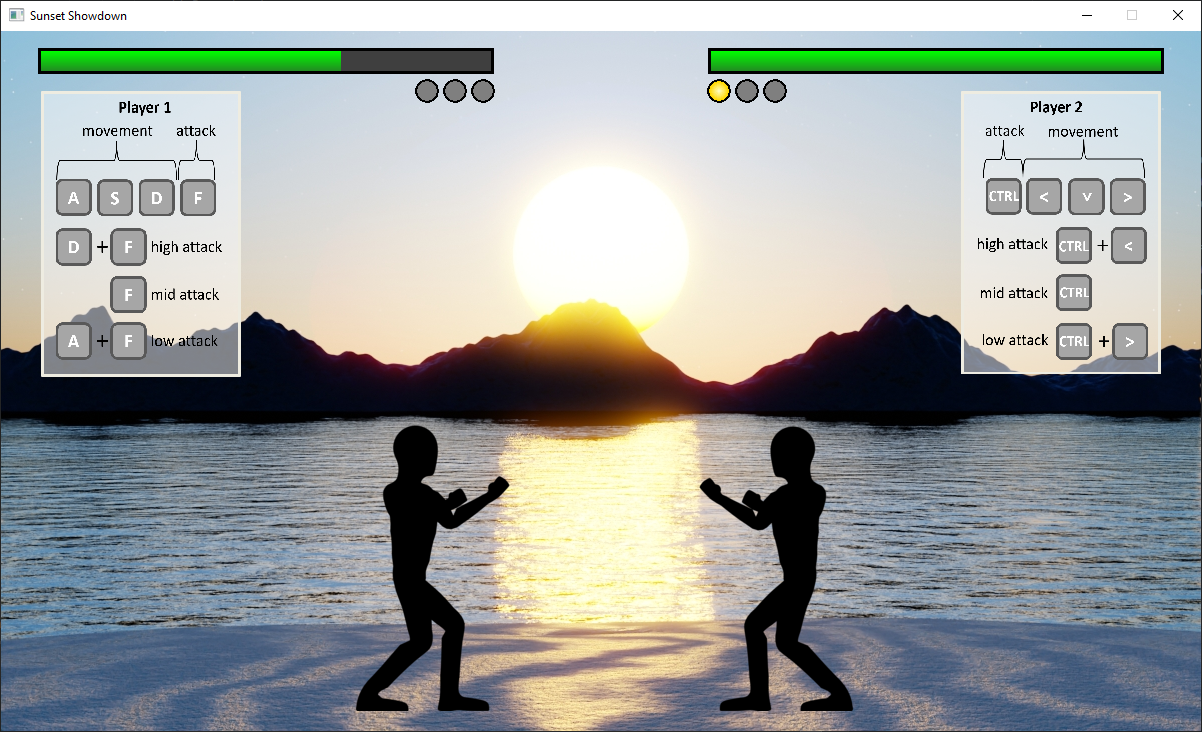
\includegraphics[width=0.64\linewidth]{rys02/interfejs}
	\caption{Widok intefejsu użytkownika gry \emph{Sunset Showdown}}
	\label{fig:interfejs}
\end{figure}
Na rysunku \ref{fig:interfejs} przedstawiono wygląd interfejsu użytkownika gry \emph{Sunset Showdown}. Postacie graczy zobrazowane są na nim jako sylwetki w jednolitym, czarnym kolorze. W górnej części ekranu znajdują się zielone paski zdrowia dla każdego z graczy. Zmniejszają się one w miarę otrzymywania obrażeń przez postacie. Poniżej pasków zdrowia znajdują się ikony w kształcie kółek. Jeżeli są zapalone na żółto, to wskazują na wygrane rundy.

Po bokach ekranu umiejscowione są schematy sterowania dla każdego z graczy, przedstawiające przypisane klawisze i ich funkcje w grze. Dla Gracza 1, po lewej stronie, przyciski 'A', 'S', 'D', i 'F' odpowiadają za ruchy i podstawowe ataki, z dodatkowymi kombinacjami klawiszy dla ataków wysokich, średnich i niskich. Analogicznie, Gracz 2, po prawej stronie ekranu, korzysta z klawiszy strzałek oraz 'CTRL' do sterowania swoją postacią i wykonania ataków.

\section{Tryby gry}
W \emph{Sunset Showdown} dostępne będą dwa podstawowe tryby gry. Tryb offline umożliwi dwóm graczom wspólną rozgrywkę na jednym komputerze przy użyciu tej samej klawiatury. Oprócz tego gra będzie oferować tryb online, który pozwali graczom na połączenie się przez Internet z osobnych komputerów. W tym trybie gracze będą mogli tworzyć pokoje gry, do których dostęp jest możliwy po wprowadzeniu specjalnego kodu pokoju. Aby założyć pokój, niezbędne będzie połączenie komputera do routera z aktywną opcją Universal Plug and Play (UPnP). Natomiast dołączenie do pokoju będzie wymagało jedynie standardowego połączenia internetowego. Funkcje te będą dostępne w menu głównym gry.



% TO DO: Proszę dopisać podrozdział o narzędziach, środowiskach i technologiach, jakie Pan miał zamiar wykorzystać podczas realizacji pracy.
% Generalnie brakuje też informacji o wymaganiach systemowych, infrastrukturze itp.
% Poza tym warto dodać, że podczas implementacji planował Pan skorzystać z wersjonowania kodu itp.
% W pracy dyplomowej można się chwialić wszystkimi zrobionymi rzeczami (sukcesami i porażkami też).

% TO DO: Proszę rozszerzyć wykaz literatury. Jedynie dwie pozycje to trochę za mało (podczas recenzowania bierze się pod uwagę dobór źródeł!!!!).
% Może Pan zacytować książki dotyczące wykorzystanych technologii, jak również dokumenację techniczną i strony projektów bibliotek i frameworków

